\documentclass[tc, manuscript]{copernicus}

\usepackage{booktabs}
\usepackage{multirow}
\usepackage{siunitx} %for SI units

\begin{document}

\title{Fountain scheduling strategies to improve water use efficiency of artificial
ice reservoirs (Icestupas)}

\def\Authors{Suryanarayanan Balasubramanian\,$^{1,2}$, Martin Hoelzle\,$^{1}$Roger Waser\,$^{3}$,Martin Von Burg\,$^{3}$,}
\def\Address{$^{1}$University of Fribourg, Department of Geosciences, Fribourg, Switzerland $^{2}$University of
Applied Sciences and Arts, Luzern, Switzerland} \def\corrAuthor{Suryanarayanan Balasubramanian}
\Author[1,2]{Suryanarayanan}{Balasubramanian}
\Author[1]{Martin}{Hoelzle}
\Author[3]{Roger}{Waser}
\Author[3]{Martin}{Von Burg}
\affil[1]{University of Fribourg, Department of Geosciences, Fribourg, Switzerland}
\affil[2]{Himalayan Institute of Alternatives, Ladakh, India}
\affil[3]{University of Applied Sciences and Arts, Luzern, Switzerland}

\correspondence{suryanarayanan.balasubramanian@unifr.ch}

\runningtitle{Scheduling AIR fountains}

\runningauthor{S. Balasubramanian}

\firstpage{1}

\maketitle

\begin{abstract}

  Artificial Ice Reservoir (AIR), often also called - Ice Stupa - are a climate adaptation strategy developed in the Indian Himalayas (Ladakh). With this technology, otherwise unused stream or lake water is stored in large ice towers in winter. The melt water that is then available in spring is used for irrigation in agriculture when the melt water from glaciers is still not sufficient. Recent studies have shown that during construction of traditional AIRs over 75 \% of the water sprayed was lost. Therefore, fountain wastewater production have to be reduced to improve water use efficiency. Improved fountain scheduling was realized using an automation system that computes recommended discharge rates using real-time weather inputs and location metadata. During the winter of 2021-22, a traditional and an automated AIR were built in Guttannen, Canton of Berne, Switzerland with the main aim of comparing and quantifying the benefits of using such automation systems.
  The scheduled fountain produced similar ice volumes while consuming 87 \% lesser water than the unscheduled fountain. Overall, these results show that scheduled fountains can increase the water use efficiency without compromising on meltwater production.

\end{abstract}

\introduction

In some arid mountain regions the lack of glacier melt water during the irrigation season is the main constraint on agricultural production. As the area irrigated is often governed by the limited availability of water or labour to carry water, there is much interest at the village level in adopting water storage techniques. One of such a technique has gained many
users, particularly farmers, is called artificial ice reservoirs (AIRs) or ice stupas. These AIRs are traditionally constructed by diverting glacial streams into fountain spray systems via embankments and pipelines. However, traditional construction strategies are prone to pipeline freezing events that increase the manual effort required to maintain the AIRs. Moreover, this strategy uses unscheduled fountains that spray all the available water all the time, thereby resulting in low water use efficiency. Improvement of these construction strategies, therefore, will allow the farmers to cultivate larger areas or to devote more time to other activities. 

Fountain scheduling methods are one option for reducing watering volumes for AIR construction systems and, at the same time, increase water use efficiency. The goal of fountain scheduling is to make the most efficient use of water by spraying the correct amount of water at the right time making water available, when the AIR
surface really can freeze it. We expect scheduled fountains to produce higher water use efficiency since they produce lower fountain wastewater. Additionally, lower fountain wastewater productions also lowers the melting energy resulting in higher ice volumes.

However, manually adjusting and scheduling fountains is unrealistic. Firstly, constant adjustments of discharge rates in response to the significant diurnal and seasonal variations of the freezing rates is impractical. Secondly, frequent pipeline water drainage is required to prevent freezing events during scheduled fountain
disuse intervals is unfeasible. Therefore, operation of scheduled fountains via automation systems would be a large improvement of the AIRs and should be certainly further enhanced.

Proper fountain scheduling systems require responses to two following questions:

(a) When should the water be turned on and off?
(b) How much water should be sprayed?

For answering these questions an extended knowledge of the surface freezing rates are important. Surface freezing rates can be calculated by the evaluation of the full energy balance model \cite{balasubramanianInfluenceMeteorologicalConditions2022} and \cite{oerlemansBriefCommunicationGrowth2021}.
However, in order to produce recommended discharge rates, a reduced version of the full energy balance model is developed seeking a balance between model complexity and data availability in order to produce recommended discharge rates for the automation system efficiently.

The main interest in using model results is to simulate fountain schedules relative to various constrains in capital investments, construction duration as well as in water availability. The fountain scheduling strategies are evaluated from the relative water use efficiency and maximum ice volume produced during the construction period. The specific objectives of this study include the presentation of the automation system construction and examples of its application to the computation of fountain scheduling strategies.

\section{Study site and data}

The Guttannen site (46.66 $\degree$N, 8.29 $\degree$E) is situated in the Berne region, Switzerland and has an altitude of 1047 $m$ a.s.l. In the winter (Oct-Apr), mean daily minimum and maximum air temperatures vary between -13 and 15 $\degree C$. Clear skies are rare, averaging around 7 days during winter. Daily winter precipitation can sometimes be as high as 100 $mm$. These values are based on 30 years of hourly weather model simulations \citep{guttannen}. Two AIRs were constructed by the Guttannen Bewegt Association, the University of Fribourg and the Lucerne University of Applied Sciences and Arts during the winters of 2021-22 using a traditional and an automated construction strategy.

\begin{figure}[t]
\includegraphics[width=8.3cm]{Figures/2AIRs.jpg}
\caption{Automated and traditional AIRs  at Guttannen on February 6, 2022. Picture credits: Daniel Bürki}
\label{fig:2AIR} 
\end{figure}

In order to compare both the construction strategies, the automated and the traditional AIRs were constructed adjacent to each other as shown in Fig. \ref{fig:2AIR}. This ensured both AIRs shared the same water source and similar weather patterns. In addition, a webcam guaranteed a continuous survey of the automated AIR.   

In the traditional strategy, tree branches were laid covering the fountain pipe to initiate and speed up of generating a fast ice cone formation process. The fountain discharge was maintained at maximum and its height was increased from 3 to 6\,$m$ during the construction period.

In the automated strategy, only the fountain pipe was placed before the water spray started. A programmed automation system controlled the fountain discharge rate during the whole winter season using real time weather input and several control parameters, which could be tested and controlled via a data logger user interface. 

\subsection{Meteorological data}
Air temperature, relative humidity, wind speed, pressure, longwave, shortwave direct and diffuse radiation are required to calculate the surface energy balance of an AIR (see Fig. \ref{fig:aws}). The construction period starts when the fountain was first switched on and ends when the fountain was last switched off. These two dates are denoted as start and fountain off dates henceforth.

\begin{figure*}[t]
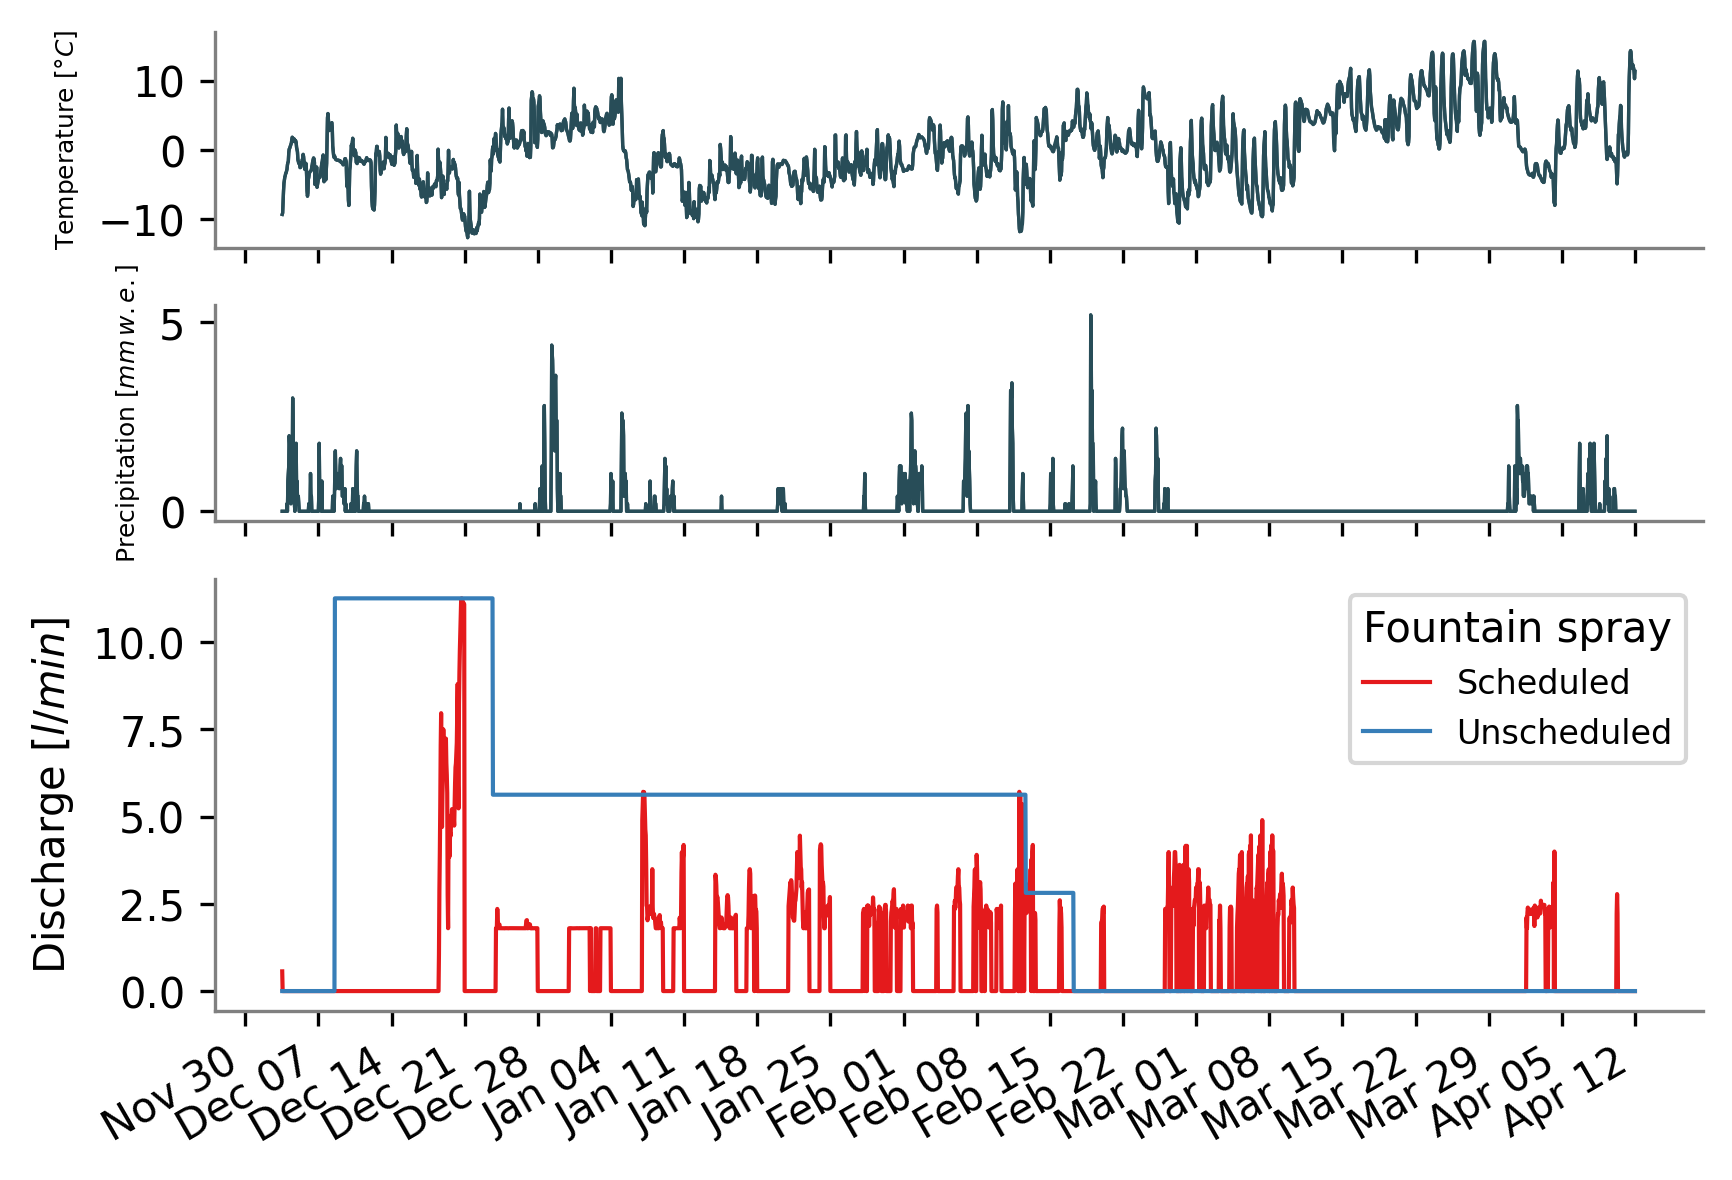
\includegraphics[width=12cm]{Figures/data.png}
\caption{Temperature, precipitation and discharge measurements at the Guttannen construction site}
\label{fig:aws} 
\end{figure*}

The weather data source was an automatic weather station (AWS) located around 20 m away as shown in Fig. \ref{fig:2AIR}. Less than 0.4 \% of the data was found to be corrupted and these were filled by linear interpolation. 
We define the fountain used through four attributes by the spray radius, the discharge rate, the pipe height and the water temperature.

\subsection{Fountain observations}

 The spray radius $r_F$ was estimated from the mean AIR circumference measured in the drone surveys during the fountain runtime. The discharge rate of the scheduled fountain was measured by the automation system. The discharge of the unscheduled fountain was using the maximum discharge rate recorded by the automation system. This was because the unscheduled fountain has been spraying the maximum discharge rate during the full construction period. However,
the discharge rate was reduced by half whenever a new pipe of 1 m length was installed to increase the fountain height. The same reduction in magnitude was also well observed for the scheduled fountain discharge rate. Therefore, we determine the discharge of the traditional fountain by using the measurements of the discharge rate for the automated fountain. A new fountain design was used for the automated strategy since the traditional fountain design was unable to function in the whole range of discharge rates suggested by the automation system.


\subsection{Drone surveys}

Several photogrammetric surveys were conducted on the traditional and the automated AIRs. The details of these surveys and the methodology used to produce the corresponding outputs are explained in the Appendix. The digital elevation models (DEMs) generated from the obtained imagery were analysed to document the spray radius, the surface area and the volume of the ice structures. The number of drone surveys conducted for the traditional and the automated AIRs were 6 and 3, respectively (see Table). The last drone flight was used to set the dome volume for the traditional AIR. The dome volume for the automated AIR represented the snow volume found before the fountain was switched on. The remaining surveys were used for model validation.

\begin{table}
	\centering
	\caption{ Summary of the drone surveys}
	\label{tab:uav}
	\begin{tabular}{@{}|llllll|@{}}
		\toprule
		\textbf{}              & \textbf{No.} & \textbf{Date} & \textbf{Volume} & \textbf{Radius} & \textbf{Surface Area} \\ \midrule
		\multicolumn{1}{|l|}{\multirow{6}{*}{\rotatebox[origin=c]{90}{Traditional}}}
		                       & 1            & Dec 23, 2021  & 17 $m^{3}$     & 2.9 $m$
		                       & 47 $m^{2}$                                                                      \\
		\multicolumn{1}{|l|}{} & 2            & Jan 3, 2022  & 22 $m^{3}$     & 3.4 $m$
		                       & 61 $m^{2}$                                                                      \\
		\multicolumn{1}{|l|}{} & 3            & Jan 22, 2022   & 626 $m^{3}$     & 4 $m$
		                       & 79 $m^{2}$                                                                      \\
		\multicolumn{1}{|l|}{} & 4            & Feb 6, 2022  & 44 $m^{3}$     & 4.2 $m$
		                       & 86 $m^{2}$                                                                      \\
		\multicolumn{1}{|l|}{} & 5            & Feb 12, 2022  & 62 $m^{3}$     & 4.2 $m$
		                       & 108 $m^{2}$                                                                      \\
		\multicolumn{1}{|l|}{} & 6            & & $m^{3}$     & $m$
		                       & $m^{2}$
		\\\midrule
		\multicolumn{1}{|l|}{\multirow{3}{*}{\rotatebox[origin=c]{90}{Automatic}}}
		                       & 1            & Dec 23, 2021  & 22 $m^{3}$      & 3.7 $m$
		                       & 57 $m^{2}$                                                                       \\
		\multicolumn{1}{|l|}{} & 2            & Jan 3, 2022   & 30 $m^{3}$      & 3.9 $m$
		                       & 66 $m^{2}$                                                                       \\
		\multicolumn{1}{|l|}{} & 3            &               &    $m^{3}$      &     $m$
		                       &    $m^{2}$                                                                       \\
		\bottomrule
	\end{tabular}

\end{table}

\subsection{Bulk temperature measurements}

Eight thermistors recorded temperature variations across the interior of the Automated Guttannen AIR. 

\section{Methods}

\subsection{Automation system}

\subsubsection{Automation hardware}

The automation system implements fountain scheduling strategies for the twin objectives of ice volume (ICV) and water use efficiency (WUE). The ICV objective is suitable at locations with sufficient water volumes to
freeze during the construction period. The WUE objective is suitable at locations with favourable weather conditions constrained by available water supply. For the ICV objective, the model assumptions overestimate the freezing rate whereas for the WUE objective the model assumptions underestimate the freezing rate. 

The automation hardware consists of an AWS, flowmeter, control valve, drain valves, air valves, fountain, pipeline and a logger. The logger feeds the AWS data to the automation software and informs the recommended discharge rate to the flowmeter. The flowmeter adjusts the control valve to match the
recommendation. However, the recommended discharge rate is ignored if any of the termination criterion are valid. The termination criterion prevent water loss and pipeline freezing events. In case a termination criteria is valid, the drain and air valves empty the water in the pipeline.

\subsubsection{Automation software}

The automation software uses several assumptions to reduce the data requirement of the energy balance model. The assumptions are categorised into two cases based on whether they favour higher WUE or ICV and are described in the Appendix and summarised in Table \ref{tab:assumptions}.  

\begin{table}[]
\centering
\caption{Assumptions introduced to simplify the model.}
\label{tab:assumptions}
\begin{tabular}{@{}lllll@{}}
\toprule
\textbf{Estimation of} & \textbf{Symbol} & \textbf{ICV Assumptions} & \textbf{WUE Assumptions} & \\ \midrule
\multicolumn{1}{|l}{Surface Area}        & $A_{cone}$ & $ \sqrt{2} \pi r_{F}^2$ & $\pi r_{F}^2$ & \multicolumn{1}{l|}{} \\ \midrule
\multicolumn{1}{|l}{Shortwave Radiation} & $q_{SW}$ & $cld = 0$ ; $\alpha=\alpha_{snow}$; & $cld = 1$ ;
$\alpha=\alpha_{ice}$; & \multicolumn{1}{l|}{} \\ 
\multicolumn{1}{|l}{ } &  & $f_{cone} = \frac{cos \theta_{sun} + \pi sin \theta_{sun}}{2\sqrt{2}\pi}$  & $f_{cone} = sin \theta_{sun} / 2$ & \multicolumn{1}{l|}{} \\ \midrule
\multicolumn{1}{|l}{Longwave Radiation}  & $q_{LW}$ & $cld = 0$ ; $T_{ice} = 0$ & $cld = 1$ ; $T_{ice} = 0$ & \multicolumn{1}{l|}{} \\ \midrule
\multicolumn{1}{|l}{Sensible and Latent Heat}       & $q_{S}$ &$\mu_{cone} = 1.5$  & $\mu_{cone} = 1$ & \multicolumn{1}{l|}{} \\ \midrule
\multicolumn{1}{|l}{Temperature heat flux} & $q_{T}$ & 0 & 0 & \multicolumn{1}{l|}{} \\ \midrule
\multicolumn{1}{|l}{Fountain discharge heat flux} & $q_{F}$ & 0 & 0 & \multicolumn{1}{l|}{} \\ \midrule
\multicolumn{1}{|l}{Ground heat flux}    & $q_{G}$ & 0 & 0 & \multicolumn{1}{l|}{} \\ \bottomrule
\end{tabular}
\end{table}

Using the simplifications shown in Table \ref{tab:assumptions}, we can compute the expected freezing rate or recommended discharge rates using the following set of equations:

\begin{subequations}
	\begin{align}
		\label{eqn:T}
   \frac{q_{SW} + q_{LW} + q_{S}}{\rho_w \cdot L_F} + \frac{q_L}{\rho_w \cdot L_V} & \approx f(hod, T_a, RH,
   v_a) \\
		\label{eqn:auto}
  Q_{F} & \approx f(hod, T_a, RH, v_a) \cdot \pi r_{F}^2 \cdot
  \frac{1000}{60}
	\end{align}
\end{subequations}

where $r_F$ is the fountain spray radius, $Q_{F}$ is the discharge rate, f is the simplified energy balance function and $hod$ is the hour of day.

Equation \ref{eqn:auto} is implemented in the automation system through a user interface that enables input of the spray radius, altitude, latitude and longitude of the construction location. Once switched on, the automation system regulates the fountain discharge rate based on the recommended discharge rate. However, certain termination criterion override the recommendation of the discharge rates  to prevent water loss and pipeline freezing events. These criterion are listed in the below items: 

\begin{itemize}

\item Loss of water droplets due to high wind speed are avoided by introducing a wind speed limit 

\item Pipeline freezing events due to very cold conditions are avoided by setting a minimum temperature limit 

\item Pipeline damage is avoided by draining the pipeline upon a pipeline freezing event detection. Pipeline freezing events are assumed if $Q_F = 0$ for at least 20 seconds.

\item Water loss is avoided by detection of pipeline leakage/damage. Pipeline leakage is assumed if $Q_F > Q_{leak}$. 

\item Pipeline freezing events are prevented by ignoring low discharge rate recommendations  

\end{itemize}

\subsection{Calibration}
We retain the default values of all parameters used in \cite{balasubramanianInfluenceMeteorologicalConditions2022} for our analysis.  

In addition, two model variables, fountain water temperature ($T_F$) and AIR density ($\rho_{AIR}$) are parametrised. Both variables were assumed to be constant in the previous versions of the model. With the extended measurement dataset of CH22 AIR, we estimate the water temperature variable by assuming it is equal to our ground temperature measurements but only when the air temperature was not subzero. Under subzero conditions, the water droplets are likely to cool to 0 C during their flight time. Therefore, the fountain water temperature was instead determined as follows:

\begin{equation}
	T_{F} = \left\{ \begin{array}{ll}
		0 & \textit{ if } T_{temp} < 0 \\
		T_{G} & \textit{ otherwise}
	\end{array} \right.
\end{equation}

where $T_{G}$ is the measured ground temperature.

The snowfall mass input of CH22 AIR was comparable to the mass input via the fountain discharge. Therefore, we could no longer assume that the AIR density was equal to ice density. We instead parameterised AIR density $\rho_{AIR}$ as follows:

\begin{equation}
  \rho_{AIR} = \frac{M_{F} + M_{dep} + M_{ppt}}{(M_{F} + M_{dep})/\rho_{ice} + M_{ppt}/\rho_{snow}}
\end{equation}

where $M_F$ is the cumulative mass of the fountain discharge; $M_{ppt}$ is the cumulative precipitation; $M_{dep}$ is the cumulative accumulation through water vapour deposition; $\rho_{ice}$ is the ice density (917 $kg\,m^{-3}$) and $\rho_{snow}$ is the density of wet snow (300 $kg\,m^{-3}$) taken from
\cite{cuffeyPhysicsGlaciers2010} .

\subsection{Validation}
We performed the validation of the physical model on the two different AIRs using two different datasets. The AIR mean temperature and ICV measurements. This was because there were fewer successful ICV measurements for the automated AIR due to  a lack of reference points on the snow covered structure to create a fully correct geo-referenced ground control. Meanwhile, the traditional AIR being steeper exposed that resulted with much more ICV measurements. However, for this ICV, we did not have an AIR mean temperature dataset. Therefore, the calibrated physical model was tested using the hourly AIR mean temperature measurements for the automated AIR and the ICV measurements for the traditional AIR, respectively. Root mean squared error (RMSE) and correlation coefficient served as the evaluation metric in both the cases. Hourly AIR mean temperature measurements were produced from the mean of all the six thermistor measurements located at the
interior of the AIR throughout the construction duration. Mean AIR temperature was estimated to be the modelled average of surface temperature $T_{ice}$ and bulk temperature $T_{bulk}$. Ice volume was recorded using several
 drone surveys as shown in Table \ref{tab:uav}.

The performance of the ICV and WUE versions of the physical model was assessed by comparing its discharge rate estimates with the validated freezing rate of the calibrated physical model.

\section{Results}

\subsection{Energy balance model validation}
The physical model achieved an RMSE of $4 \degree C$ with the AIR mean temperature measurements of the automated AIR and an RMSE of $m^3$ with the ice volume measurements of the traditional AIR. The estimated and measured AIR
mean temperatures and ice volumes are shown in Fig. \ref{fig:validation}
 
\begin{figure*}[t] 
  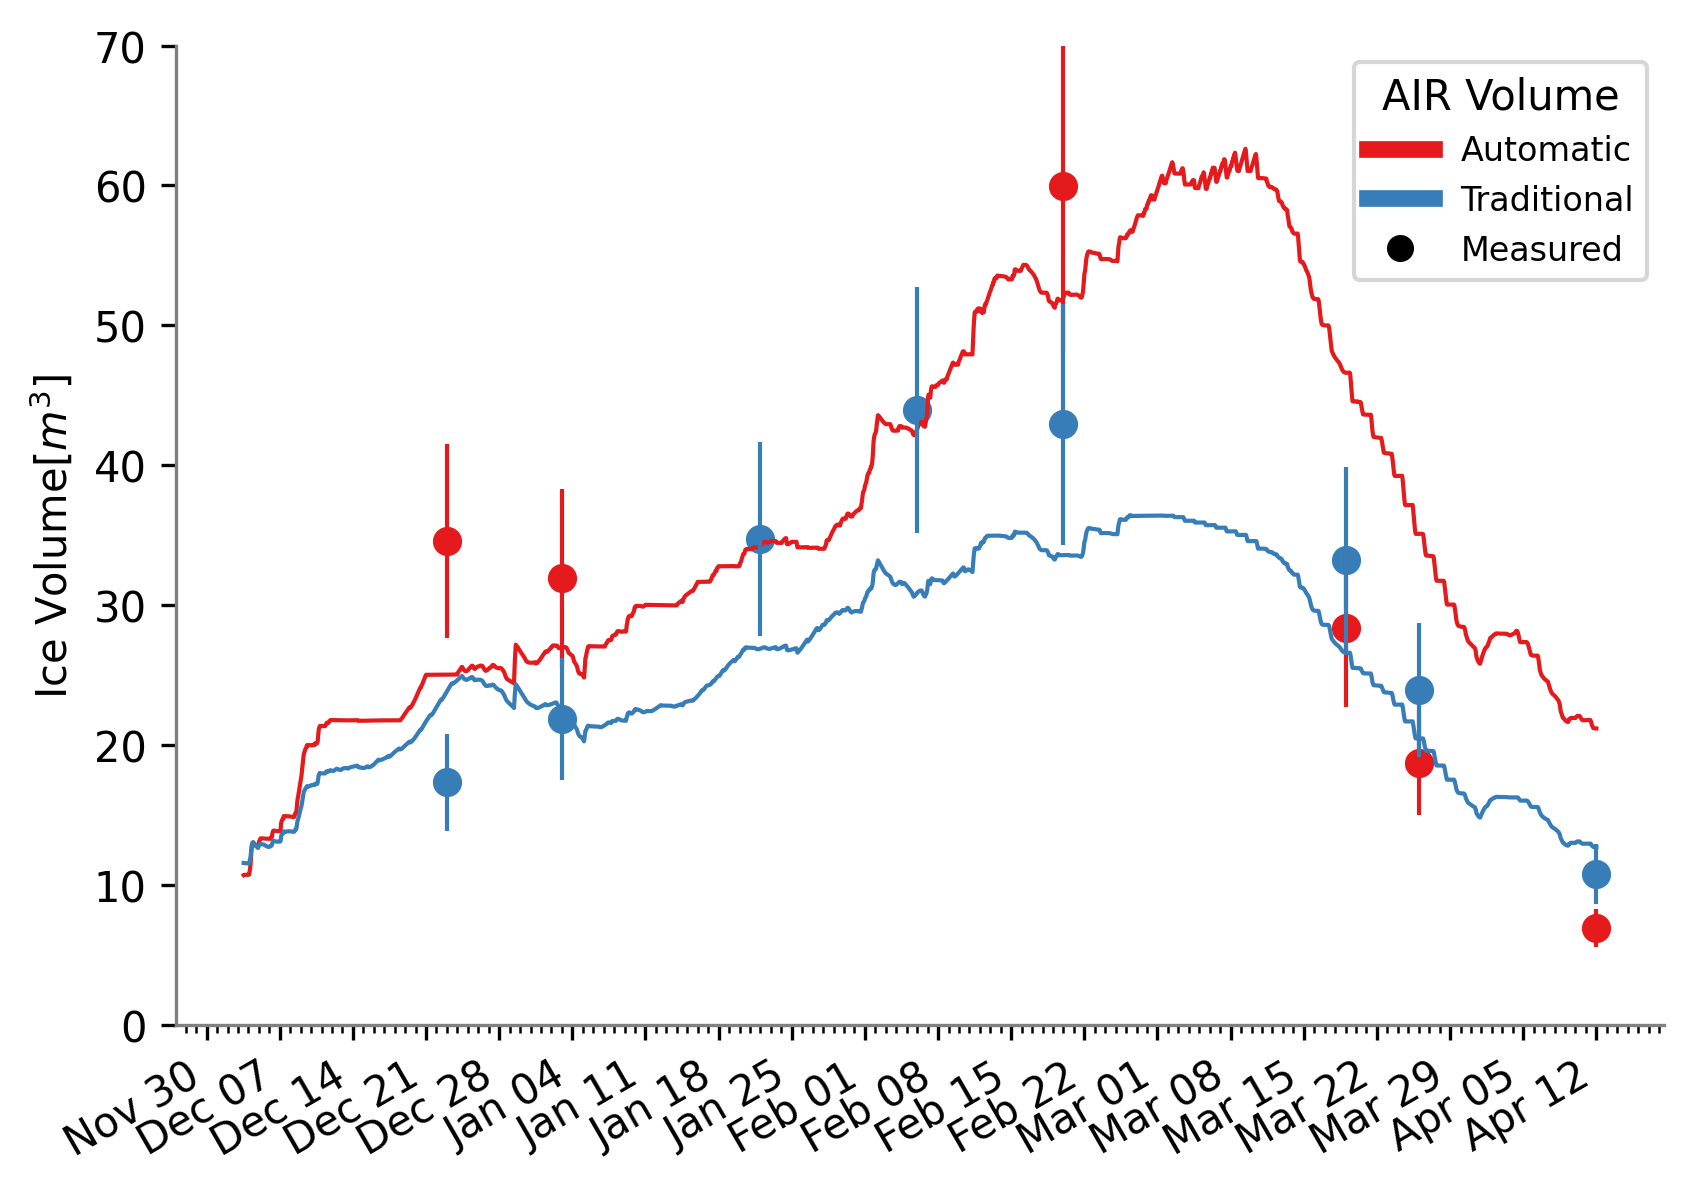
\includegraphics[width=12cm]{Figures/validation.png} 
  \caption{Bulk temperature and ice volume validation of the scheduled and unscheduled fountain construction strategies.} 
\label{fig:validation} 
\end{figure*}

\subsection{Scheduled discharge rate estimation}

We found that the simplified energy balance model estimated the freezing rate of the unscheduled fountain with a correlation higher than 0.5 and RMSE less than 1 $l/min$ for both the ICV and WUE objectives. The ICV scheduled fountain overestimated the freezing rate 90 \% of the construction duration whereas the WUE
scheduled fountain underestimated the freezing rate 80 \% of the construction duration as shown in Fig.
\ref{fig:freezing_rate}.

\begin{figure*}[t]
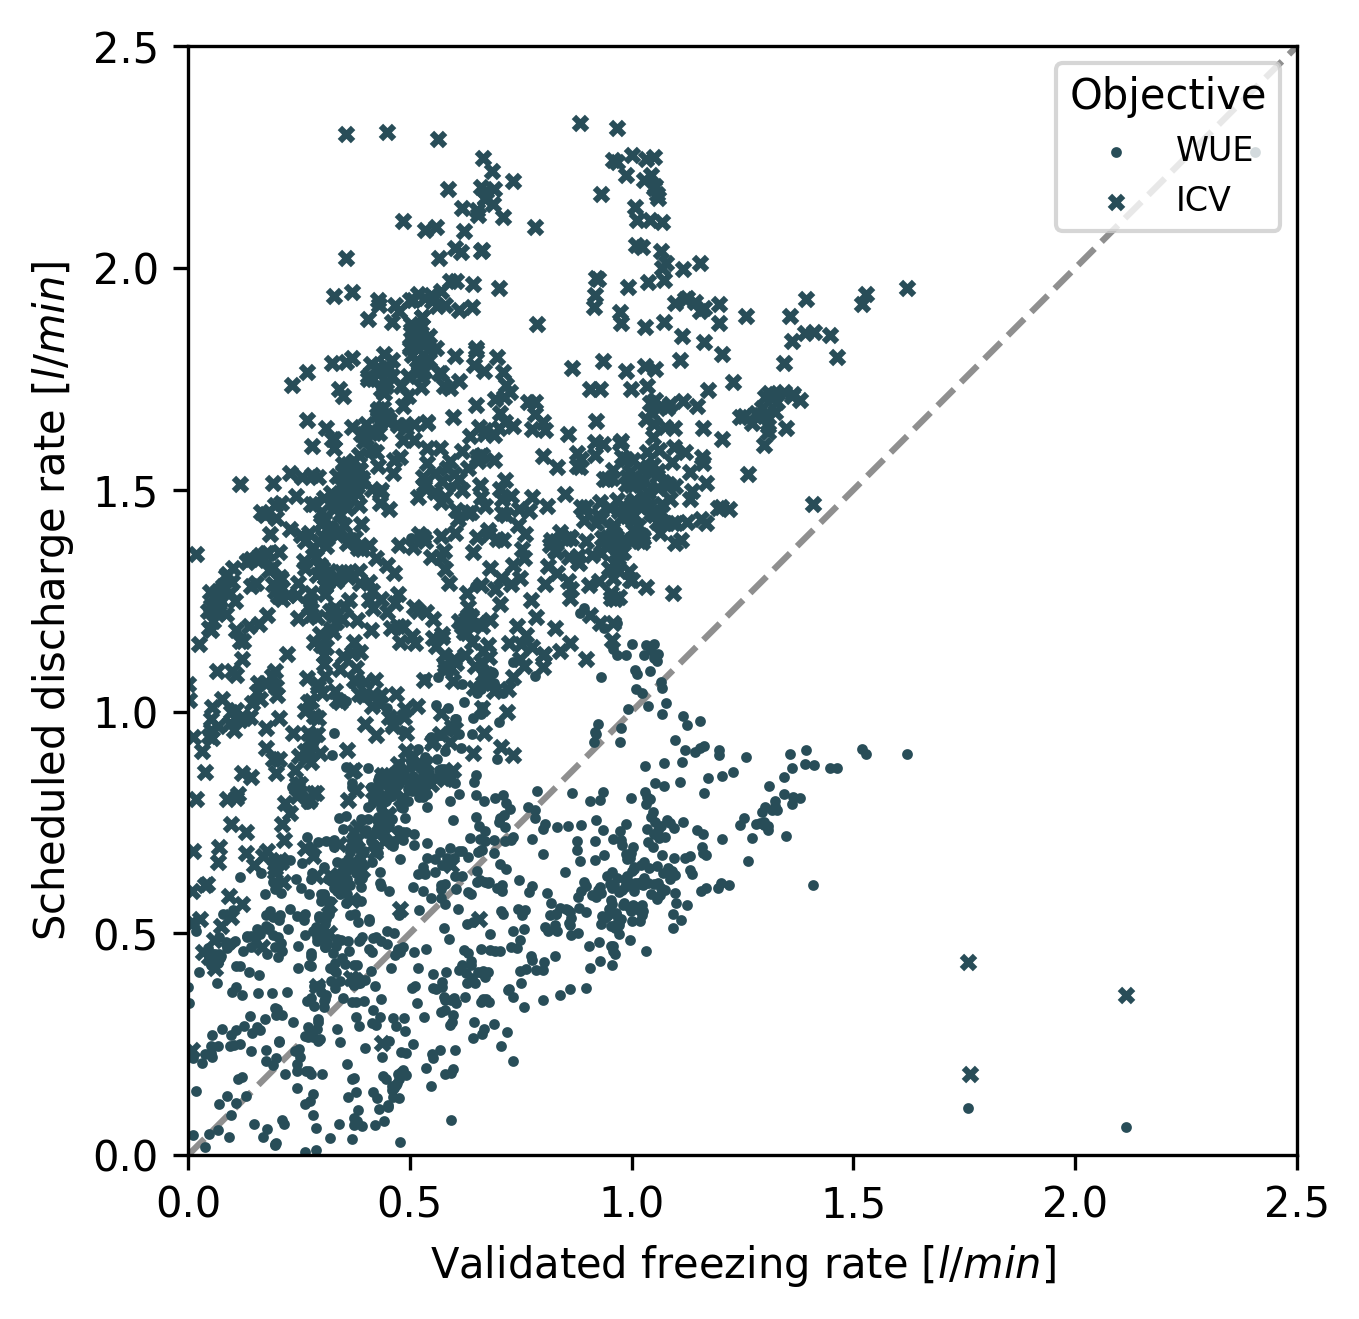
\includegraphics[width=12cm]{Figures/freezing_rate_corr.png}
\caption{Scheduled discharge rate estimates of the simplified energy balance model with the WUE and ICV
assumptions compared with the validated freezing rate of the full energy balance model.}
\label{fig:freezing_rate}
\end{figure*}

\subsection{Comparison of AIR construction strategies}

Given the excessive discharge rate of the unscheduled fountain, it is not surprising that its fountain wastewater output is an order of magnitude higher than the scheduled fountain. However, the lower measured volume of the traditional AIR, it is unexpected that it corresponds to a higher ice mass. This is because the lower snowfall input of the traditional AIR made it more dense than the automated AIR (see Table \ref{tab:mb}). 


\begin{table}
	\centering
	\caption{ Summary of the mass balance and AIR characteristics estimated at the end of the respective
  simulation duration for the automated and the traditional AIRs}
	\label{tab:mb}
	\begin{tabular}{@{}|llllll|@{}}
		\toprule
		\textbf{}              & \textbf{Name}                   & \textbf{Symbol} & \textbf{Traditional} & \textbf{Automated} &
		\textbf{Units}                                                                                                       \\ \midrule
		\multicolumn{1}{|l|}{\multirow{3}{*}{\rotatebox[origin=c]{90}{Input}}}
		                       & Fountain discharge              & $M_F$           & \num{7.3e5}   & \num{7.5e4}     & $kg$  \\
		\multicolumn{1}{|l|}{} & Snowfall                        & $M_{ppt}$       & \num{1.3e4}   & \num{2.2e4}   & $kg$  \\
		\multicolumn{1}{|l|}{} & Deposition                      & $M_{dep}$       & \num{2.3e2}   & \num{8.9e2}     & $kg$  \\ \midrule
		\multicolumn{1}{|l|}{\multirow{4}{*}{\rotatebox[origin=c]{90}{Output}}}
		                       & Meltwater                       & $M_{water}$     & \num{2.0e4} & \num{1.2e4}   & $kg$  \\
		\multicolumn{1}{|l|}{} & Ice                             & $M_{ice}$       & \num{2.2e4} & \num{3.0e4}    & $kg$  \\
		\multicolumn{1}{|l|}{} & Sublimation                     & $M_{sub}$       & \num{1.5e3} & \num{1.2e3}     & $kg$  \\
		\multicolumn{1}{|l|}{} & Fountain wastewater             & $M_{waste}$     & \num{7.0e5} & \num{6.5e4}     & $kg$  \\ \midrule
		\multicolumn{1}{|l|}{\multirow{7}{*}{\rotatebox[origin=c]{90}{Energy Balance}}}

                           & Shortwave radiation             &  $q_{SW}$       & $13 \pm 36$  & $8 \pm 24$ & $W\,m^{-2}$ \\
		\multicolumn{1}{|l|}{} & Longwave radiation              &  $q_{LW}$       & $-21\pm 30$  & $-9 \pm 23$& $W\,m^{-2}$ \\
		\multicolumn{1}{|l|}{} & Sensible heat                   &  $q_{S}$        & $1\pm 12$  & $2 \pm 17$   & $W\,m^{-2}$ \\
		\multicolumn{1}{|l|}{} & Latent heat                     &  $q_{L}$        & $-7\pm 32$  & $-1 \pm 31$ & $W\,m^{-2}$ \\
		\multicolumn{1}{|l|}{} & Fountain water heat             &  $q_{F}$        & $3\pm 6$  & $0 \pm 1$     & $W\,m^{-2}$ \\
		\multicolumn{1}{|l|}{} & Ground heat                     &  $q_{G}$        & $0\pm 1$  & $0 \pm 2$     & $W\,m^{-2}$ \\
		\multicolumn{1}{|l|}{} & Surface Area                    &  $A_{cone}$     & $56\pm 5$  & $79 \pm 4$     &$m^{2}$ \\\midrule
		\multicolumn{1}{|l|}{\multirow{2}{*}{\rotatebox[origin=c]{90}{AIR}}}

		                       & Maximum Ice Volume              &                 & 47            & 67            & $m^{3}$ \\
		\multicolumn{1}{|l|}{} & Water Use Efficiency            &                 & 5             & 38            & \% \\\midrule
	\end{tabular}
\end{table}

\section{Discussion}

\subsection{Simulations of scheduled fountains}

We evaluate the benefits of the automated construction strategies by comparing them with the traditional construction strategies used in the IN21 and CH21 locations presented in
\cite{balasubramanianInfluenceMeteorologicalConditions2022}. The difference in water use efficiency and maximum ice volumes expected between unscheduled and scheduled fountains in the three locations are presented in Fig.
\ref{fig:wue}.

\begin{figure*}[t]
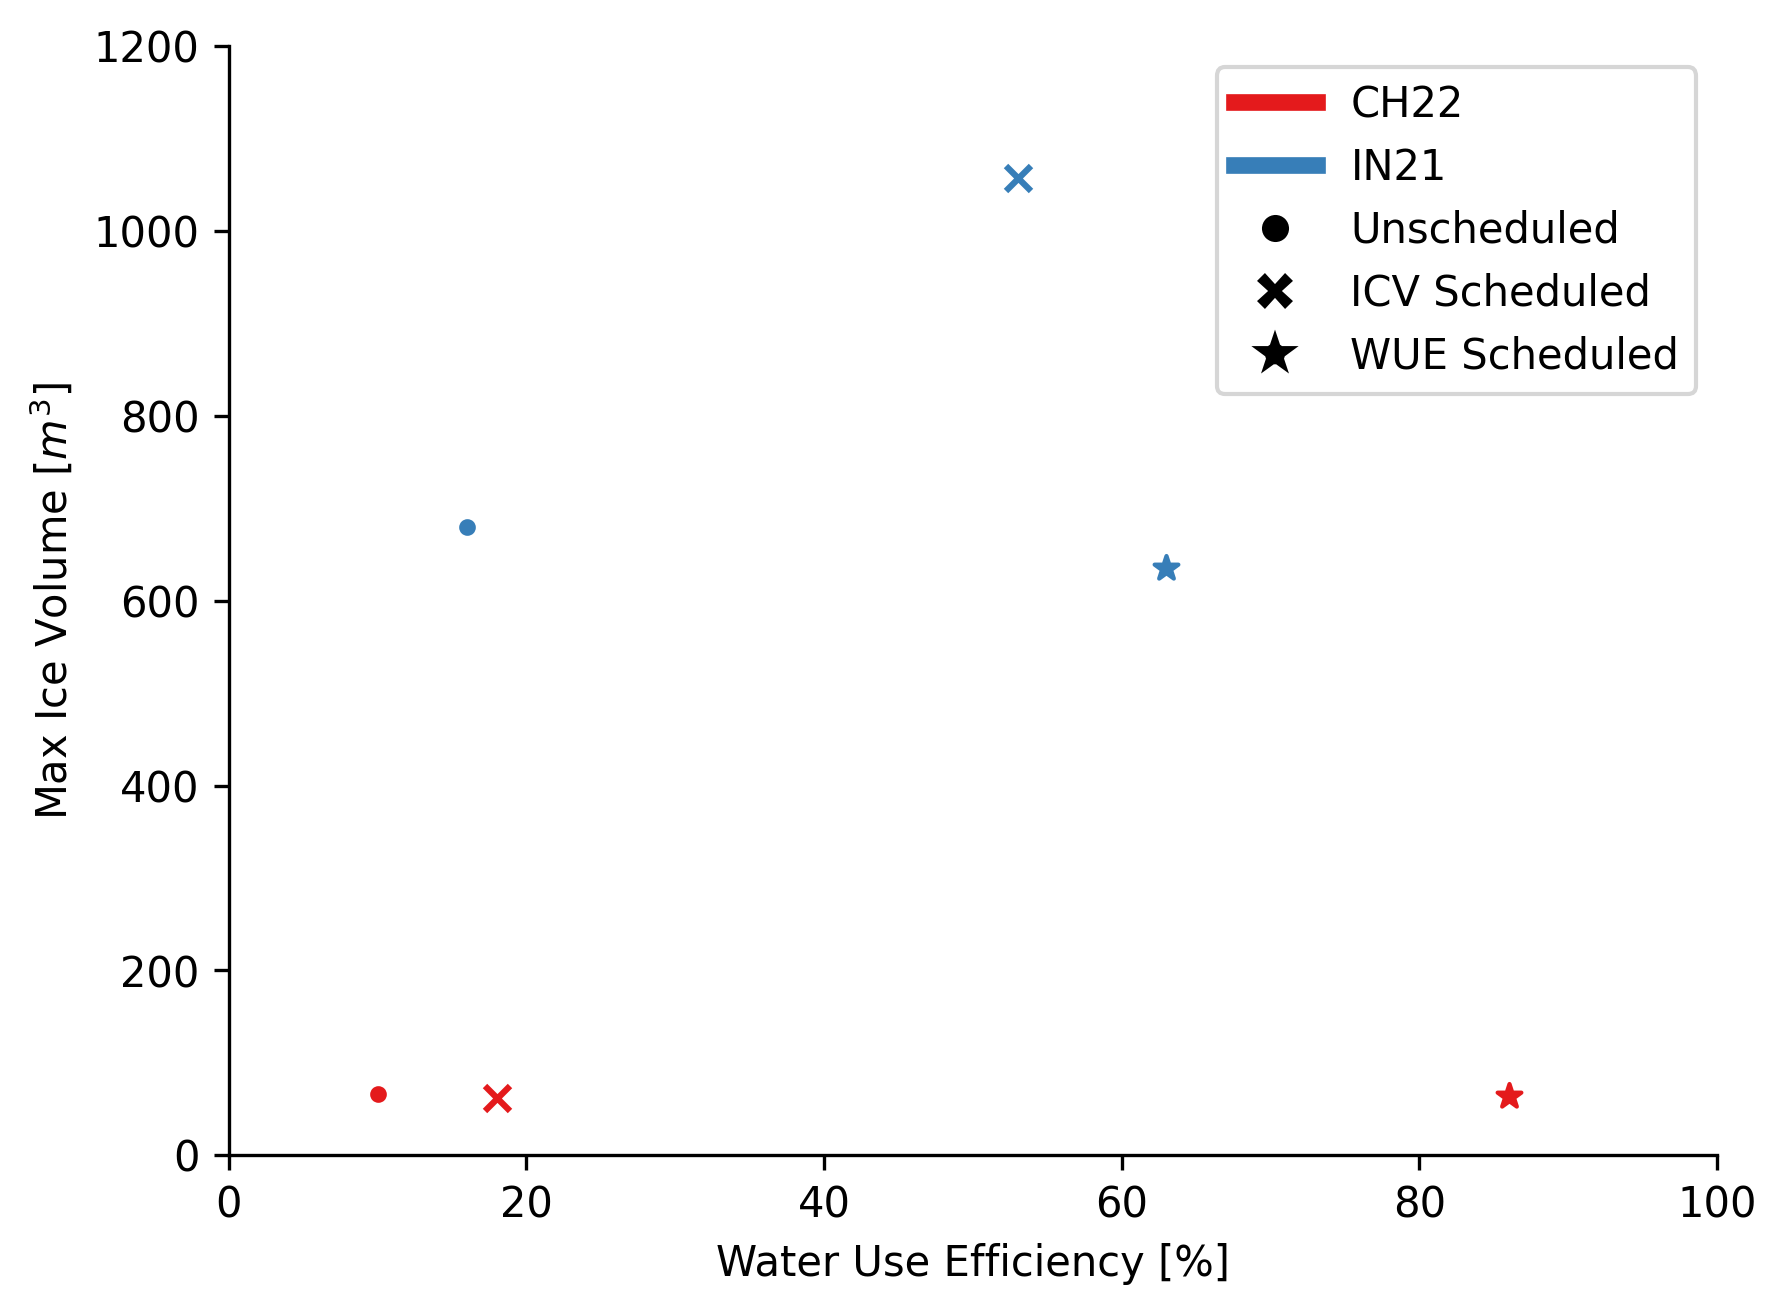
\includegraphics[width=12cm]{Figures/wue.png}
\caption{The maximum ice volume and water use efficiency estimated for the different locations and construction
strategies used}
\label{fig:wue}
\end{figure*}


\conclusions
In this paper, an automated AIR construction strategy is presented and compared with a traditional strategy
using data collected in Guttannen, Switzerland.

The main purpose of this study was to test the idea that scheduled AIR fountains could lead to a significant
improvement in water use efficiency and ice volumes. A simplified energy balance model compatible with the
limited data availability of a new location was used to produce recommended discharge rate. Nevertheless, this
model was able to capture more than 65 \% of the freezing rate variations produced by the full energy balance
model.

The automation system allows the easy handling of fountain scheduling implementation. The possibility for
changing the location and fountain metadata directly in the user interface allows tailoring the fountain
discharge rate according to the location's water supply and weather conditions. Furthermore, this construction
strategy reduces the occurence of pipeline freezing events as it drains the pipeline whenever fountain is not in
use.

Nevertheless, the real world application of this method is challenging. It is clear that if improvements are to
be achieved, future research must be devoted to modelling the impact of fountain design on the spray radius.

\appendix

\section{Simplified energy balance model}

We approximate the energy balance at the surface of an AIR by a one-dimensional description of energy fluxes as
used in \cite{balasubramanianInfluenceMeteorologicalConditions2022}. The ice volume evolution of the AIR can be
represented as: 

\begin{equation}
  \frac{\Delta V_{ice}}{\Delta t}  =  \frac{\Delta j_{cone}}{ \Delta t} \cdot A_{cone}
	\label{eqn:freeze}
\end{equation}

where $\frac{\Delta j_{cone}}{\Delta t}$ is the thickness change determined as follows:

\begin{equation}
  \frac{\Delta j_{cone}}{\Delta t}  = \frac{1}{\rho_{AIR}} \cdot (\frac{q_{SW} + q_{LW} + q_{S} + q_{F} + q_{G} -
  q_{T}}{L_F} + \frac{q_{L}}{L_V} )
	\label{eqn:freeze}
\end{equation}

Upward and downward fluxes relative to the ice surface are positive and negative, respectively. The first term
represents the surface thickness change rate due to freezing of the fountain water and melting of the ice.
$q_{SW}$ is the net shortwave radiation; $q_{LW}$ is the net longwave radiation; $q_{L}$ and $q_{S}$ are the
turbulent latent and sensible heat fluxes; $q_{F}$ is the fountain heat flux; $q_{G}$ is the ground heat flux
and $q_{T}$ is the temperature heat flux. However, we assume $q_{F}$, $q_{G}$ and $q_{T}$ to be negligible.

The data requirement was reduced by estimating the global shortwave radiation and pressure directly using the
location's coordinates and altitude through the solar radiation model described in
\citet{holmgrenPvlibPythonPython2018}. The algorithm used to estimate the clear-sky global radiation is
described in \citet{ineichenBroadbandSimplifiedVersion2008}.  

The model complexity was reduced through assumptions that optimise for the ice volume objective or the water use
efficiency objective. Assumptions are chosen based on whether they overestimate/underestimate the freezing rate.
Ice volume objective requires freezing rate to be overestimated whereas WUE objective requires freezing rate to
be underestimated. We describe these two kinds of assumptions applied on each of the energy balance components
below: 

\subsection{Surface Area $A_{cone}$ assumptions}

Since we are only interested in determination of the surface area during the accumulation period we can assume a
constant ice cone radius equal to the fountain spray radius. The surface area scales the freezing rate of the
AIR. Hence, for the ICV objective we assume the maximum possible slope of 1 for the ice cone or in other words
$h_{cone} = r_{F}$. Therefore, area is estimated as:  

\begin{equation} A_{cone} =\pi \cdot r_{F}^2 \label{eq:Area} \end{equation}

Similarly, for the WUE objective, the area of the conical AIR is approximated to the area of its circular
base.Therefore, area is estimated as:

\begin{equation} A_{cone} =\sqrt{2} \cdot \pi \cdot r_{F}^2 \label{eq:Area} \end{equation}

\subsection{Net shortwave radiation \texorpdfstring{$q_{SW}$}{Lg} assumptions}
\label{sec:SW}

The net shortwave radiation $q_{SW}$ is computed as follows:

\begin{equation} 
q_{SW} = (1- \alpha) \cdot ( SW_{direct} \cdot f_{cone} + SW_{diffuse})
\label{eqn:SW} 
\end{equation}

where $\alpha$ is the albedo value ; $SW_{direct}$ is the direct shortwave radiation; $SW_{diffuse}$ is the
diffuse shortwave radiation and $f_{cone}$ is the solar area fraction.

The diffuse and direct shortwave radiation is determined using the estimated global solar radiation as follows:

\begin{equation}
\begin{split}
  SW_{diffuse} &= cld \cdot SW_{global}\\
  SW_{direct} &= (1-cld) \cdot SW_{global}
\end{split}
\end{equation}

where $cld$ is the cloudiness factor. $cld$ is assumed to be 1 and 0 for the WUE and iceV objective
respectively.

We ignore the variations in the albedo and assume it to be equal to snow albedo and ice albedo for the iceV and
WUE objective respectively. 

The solar area fraction $f_{cone}$ of the ice structure exposed to the direct shortwave radiation depends on the
shape considered. It is computed as

\begin{equation}
		f_{cone} =\frac{(0.5 \cdot r_{cone} \cdot h_{cone}) \cdot cos \theta_{sun} +(\pi \cdot
			{(r_{cone})}^2/2) \cdot sin \theta_{sun} }{\pi \cdot r_{cone} \cdot ({(r_{cone})}^2+{(h_{cone})}^2)^{1/2}}\\
\end{equation}

For the ICV objective, since we assume the slope of the cone to be 1 $f_{cone}$ is determined
as follows:

\begin{equation}
		f_{cone} =\frac{ cos \theta_{sun} + \pi \cdot sin \theta_{sun} }{2\sqrt{2} \cdot \pi }
\end{equation}

Similarly, for the WUE objective, since we assume the slope of the cone to be negligible, we get:

\begin{equation}
		f_{cone} =\frac{ sin \theta_{sun} }{2 }
\end{equation}

\subsection{Net Longwave radiation \texorpdfstring{$q_{LW}$}{Lg} assumptions} \label{sec:LW}

We assume $T_{ice} = 0 \degree C$ in order to determine outgoing longwave radiation. Since it is challenging to
contrain the minimum ice temperature, we maintain this assumption for both our objectives. However, in order to
estimate atmospheric emissivity we again assume $cld$ to be 1 and 0 for the WUE and iceV objective respectively.

\subsection{Turbulent fluxes assumptions} \label{sec:Qs}

Turbulent fluxes estimation depend on the slope of the cone through the $\mu_{cone}$ parameter. As suggested 
by \citet{oerlemansBriefCommunicationGrowth2021}, we can estimate this parameter as follows:

\begin{equation}
  \mu_{cone} =1 + s_{cone}/2
\end{equation}

Hence, the $\mu_{cone}$ parameter takes values of 1.5 and 1 for the iceV and WUE objective respectively.  Since
turbulent fluxes impact both the freezing and the melting rates, this assumption may not favor the corresponding
objectives for certain sites.


\noappendix 

\bibliographystyle{copernicus}
\bibliography{zot_refs.bib}

\end{document}
